%No argument - what did I actually find? What is the impact?

%Bring quotes up a level - tie back to other resarch (put in discussion?)

%Poor literacy! Organize better.

%Improve / Refine themes

%Tool related benefits/challenges vs. Teaching/learning related challenges

%Why did I do semi-structured interviews?

%Limitations!

%Diagram of findings


\chapter{The Student Perspective}

In the previous chapter, we interviewed educators to discover why and how they use GitHub to augment their classes, and gained a variety of insights on the benefits and drawbacks of using such a system. These educators spoke of benefits such as the ability to monitor student work continuously and the ease with which they can reuse and remix course materials from other instructors. They also noted benefits which impact their students, such as learning how to use a tool relevant to their field, and the ability to make changes to course materials. With that, I aimed to uncover more about the student perspective, as well as to discover what challenges they may experience or concerns they may have with using GitHub for their courses. %It is important to explore the student perspective to determine the viability of GitHub and the GitHub way for education.\todo{Seems like a blanket statement. Why is it important? Hmmm, seems like you covered this at the end of the next paragraph so perhaps this statement should be removed or rewritten.}

To explore how students perceive GitHub as a learning tool, I conducted a study where GitHub was used to support the teaching and learning activities in two technical courses. The instructors would utilize GitHub in ways similar to those described by the instructors we interviewed in the previous chapter---to host course materials, projects, and assignments, and to facilitate discussion. In this study, I used exploratory questions to interview students and learn how they perceive GitHub's effectiveness as a platform for education and for their coursework.

As learning tools become more focused on student participation and contribution, it was important to place a focus on the students. By exploring the student perspective, we can determine how GitHub as a tool might help enable a participatory culture \cite{jenkins2009confronting} or serve as a tool to meet the needs of `the contributing student' model \cite{hamer2008contributing}. This may impact the development of future tools, particularly if the benefits of using GitHub are large enough to consider implementing features to support similar activities in educational tools.

\section{Research Questions}
This study explores the student perspective to gain insights on how the use of GitHub can benefit their learning, as well as how GitHub compares to the traditional learning tools students are exposed to and what GitHub provides beyond those tools. The research questions addressed during this study include:

\bigskip
\textbf{RQ1: What are computer science and software engineering student perceptions on the benefits of using GitHub for their courses?} We've seen evidence that GitHub can benefit educators in a number of ways. The natural progression was to explore student perceptions on how this tool and this way of working might also benefit them.

\bigskip
\textbf{RQ2: Will students face challenges related to the use of GitHub in their courses? If so, what are these challenges?} When adopting a new tool for a course, particularly a tool not tailored towards education, there may be some friction involved due to a lack of educationally-focused features. We aimed to identify these challenges so as to make recommendations towards designing a system more suitable for educational purposes.

\bigskip
\textbf{RQ3: What are student recommendations for instructors wishing to use GitHub in a course?} Just as there are multiple ways to use GitHub for development purposes, an educator has multiple options regarding how they can utilize GitHub as a tool for their courses. We aimed to learn what students consider to be important for instructors when creating a GitHub workflow that students would deem appropriate for their courses.
%open-ended courses
%define a workflow
%use the features

\bigskip
\textbf{RQ4: From the student perspective, how does GitHub compare to traditional Learning Management Systems?} Specifically, we aimed to discover student perceptions on currently used Learning Management Systems like Coursespaces (Moodle) and Connex (Sakai), specifically pertaining to GitHub's potential as such a portal for student interactions in their courses.

\section{Research Design}
We used a qualitative approach to study the student perspective of GitHub use in education. As Creswell \cite{creswell2013research} suggests, a qualitative and exploratory approach best suits research when a concept or phenomenon requires more understanding because there is little pre-existing research. Moreover, a qualitative approach is consistent with the previous study discussed in Chapter 4, and this is important because the aim was to investigate similar outcomes from the same phenomenon, but from another perspective. %This also continues the constructivist approach with which the research has been conducted.

Yin \cite{yin2013case} introduces case studies as ``an empirical inquiry that investigates a contemporary phenomenon within its real-life context, especially when the boundaries between phenomenon and context are not clearly evident.'' Case study design, according to Yin, should be used when (a) the study seeks to answer `how' or `why' things happen; (b) the study is focused on the natural behavior of participants; (c) the context is important for the study; or (d) there are no clear descriptions of what is happening between the phenomenon and context. Because these conditions apply to the nature of the research questions asked in this study, I chose the case study design for this work. Specifically, the study was exploratory, serving as an early investigation on the phenomenon of GitHub in the classroom and to potentially build new theories or derive new hypotheses \cite{easterbrook2008selecting}.

Specific to software engineering, Runeson \cite{runeson2012case} defines case studies as ``an empirical enquiry that draws on multiple sources of evidence to investigate one instance (or a small number of instances) of a contemporary software engineering phenomenon within its real-life context, especially when the boundary between phenomenon and context cannot be clearly specified.'' In this work, I aimed to draw from multiple sources of evidence---multiple students and instructors---to investigate the potential of using GitHub for post-secondary computer science and software engineering courses. It's important to learn student perspectives in this context and to explore the suitability of GitHub for supporting education.

\subsection{Recruitment}
The participants in this study included the main stakeholders in technical courses: the professor (the main instructor), lab instructors, and students. As the learning tools used in courses directly involve and impact these stakeholders, I wished to obtain their perspectives and opinions to answer our research questions. The aim was to explore their perspectives while the course was ongoing so that they could recall recent experiences and provide their opinions on GitHub as a learning tool.

For this study, we were opportunistic in finding cases and sought instructors who could and were willing to try using GitHub. I was able to recruit a professor who wanted to try using the tool in two different courses. Having multiple cases would allow us to explore some possible differences between the two scenarios \cite{yin2013case}. The two courses were Distributed Systems (DS), a computer science course aimed at both undergraduate and graduate students, and Software Evolution (SE), a software engineering course that was only taken by undergraduate students. Both classes were similar in size (30-40 students) and in learning activities (weekly labs and two course projects).

When the term began, I attended one of the first lectures to describe my goals and to recruit students to participate in the study. Participation was voluntary and I only contacted students if they signed up to participate---interested students signed up by providing their names and email addresses. As the course was concluding, I attended one more lecture to recruit more participants in the same manner. This method of recruitment meant that different students participated in the different phases. For example, those who responded to the preliminary survey were not necessarily interviewed.

\subsection{Research Methods}
Our study began by sending a preliminary survey to the students, asking them to discuss their opinions on learning tools in general, and on GitHub as a specific learning tool. This was distributed to all students who signed up to participate, and would guide the questions asked in the next phase.

As the main means of collecting data, I interviewed the participants who were willing to discuss their experiences and opinions. Interviewees were recruited from the participant pool who volunteered to participate during the recruitment phase. As such, respondents of the preliminary survey did not necessarily participate in future phases of data collection. Interviews began midway through the semester and continued until the conclusion of the course. Most interviews with the students were one-on-one, however, due to scheduling reasons, some students requested to be interviewed as a group of 2 or 3. Interviews with the students lasted 20-30 minutes and were all conducted face-to-face in a meeting room. Audio from every interview was recorded with participant consent, and I recorded notes for reference. The interviews were semi-structured based on 12 guiding questions (listed in Appendix B) and I probed further with additional questions as deemed appropriate. This supported the exploratory nature of the work and allowed for the discovery of interesting insights.
%citation for semi-structured interviews; runeson?

I also interviewed the course instructors: the main course instructor was interviewed at the start of the semester and after both courses concluded, and the lab instructors (one for each course) were interviewed towards the end of the course in order to find out how they utilized GitHub in their labs and to uncover their opinions on the tool's effectiveness towards the learning activities they engaged in with the students. Interviews with the instructors had a similar format to those with the students: semi-structured, 20 minutes long, with approximately 7 guiding questions (listed in Appendix B).

% \todo{add table of themes here?}

\section{Preliminary Questionnaire}
At the start of each course, a questionnaire was sent out to all students who indicated their willingness to participate during the recruitment stage. The purpose of this questionnaire was to determine the general level of experience and familiarity with GitHub, as well as to collect early impressions on GitHub as a learning tool. The questionnaire received 9 responses from the students in the SE course and 6 responses from the students in the DS course. The questions are listed in Appendix C.

Students who answered the questionnaire were generally familiar with GitHub, with only one student in both courses indicating that they were unfamiliar with the tool. The majority of respondents had not experienced courses where their instructors would use GitHub to manage course activities. When asked about how its use might benefit them, students in the DS course mainly discussed the benefits of using it for collaborating in group projects, while some raised the concern that it may not have much value for the course overall when used like an LMS. In the SE course, respondents discussed the real-world experiences using the tool would provide alongside the project collaboration advantages, as well as the public nature of projects where their work could be seen and reviewed regularly by other students and the instructors.

When asked about potential challenges, students in both courses had similar concerns, such as the implications of having publicly viewable work on cheating and plagiarism, and the lack of threaded discussions. Overall, many of the responses gathered from this questionnaire were reflective of the responses students gave during the interviews.

\section{Participants}
I conducted interviews with 13 students from SE, 1 of which was in the DS course, alongside 6 others from DS. These interviews began at the midway point of the semester and concluded at the end of the semester. The main distinction between the two courses was that SE was an undergraduate Software Engineering (SENG) course whereas DS was a Computer Science course with a mix of undergraduate and graduate students. Otherwise, the courses were laid out in a similar manner (as outlined below in Section 5.5). Table \ref{table:interviews:students} summarizes the students who participated in interviews.

% \todo{table of participants}
\begin{table}[h]
    \vspace{1pt}
        \caption{Participants and their Prior Experience with GitHub}\label{table:interviews:students}
    \vspace{1pt}
    \begin{center}
        \begin{tabular}{c | c | c}
            \hline
            ID & Prior GitHub Experience & Degree Type \\
            \hline
            DS1 & Inexperienced & Graduate \\ \hline
            DS2 & Used Academically, Professionally & Graduate \\ \hline
            DS3 & Used Academically, Professionally & Graduate \\ \hline
            DS4 & Inexperienced & Graduate \\ \hline
            DS5 & Used Academically & Graduate \\ \hline
            DS6 & Used Academically & Graduate \\ \hline
            SE1 & Used Academically, Professionally & Undergraduate \\ \hline
            SE2 & Inexperienced & Undergraduate \\ \hline
            SE3 & Used Professionally & Undergraduate \\ \hline
            SE4 & Inexperienced & Undergraduate \\ \hline
            SE5 & Used Personally & Undergraduate \\ \hline
            SE6 & Used Academically & Undergraduate \\ \hline
            SE7 & Used Professionally & Undergraduate \\ \hline
            SE8 & Inexperienced & Undergraduate \\ \hline
            SE9 & Used Professionally & Undergraduate \\ \hline
            SE10 & Used Casually & Undergraduate \\ \hline
            SE11 & Used Professionally & Undergraduate \\ \hline
            SE12 & Used Academically & Undergraduate \\ \hline
            SE13 & Used Academically & Undergraduate \\ \hline
        \end{tabular}
    \end{center}
\end{table}

\subsection{Data Analysis}
Following the interviews, I carefully transcribed every interview, then read and re-read the content for familiarity, noting important sections or responses. Next, I coded the data by labeling various segments based on the research questions of the study. Afterwards, I identified themes and concepts that surfaced multiple times. After separating the themes into well-defined categories, I compiled a final list of themes.

%table here
%DS1 - P1
%DS2 - P5
%DS3 - P7
%DS4 - P8
%DS5 - P9
%DS6 - P15 R

%SE1 - P2
%SE2 - P3
%SE3 - P4
%SE4 - P6
%SE5 - P10
%SE6 - P11
%SE7 - P12
%SE8 - P13
%SE9 - P14
%SE10 - P16
%SE11 - P17
%SE12 - P18
%SE13 - P19

\section{How GitHub was used}
The professor opted to utilize GitHub in the same way for both courses, using its features in three pivotal ways: material dissemination through the course repository, lab work through the `Issues' feature, and project hosting through various repositories. The advanced use cases we discussed in Chapter 4, such as utilizing pull requests and assignment submissions, were not used for these courses. The main course instructor was aware of some of these features but was not comfortable using GitHub beyond their knowledge.

\begin{figure}[h!]
 \caption{The front page of the SE Course Repository---the course schedule}
 \centering
   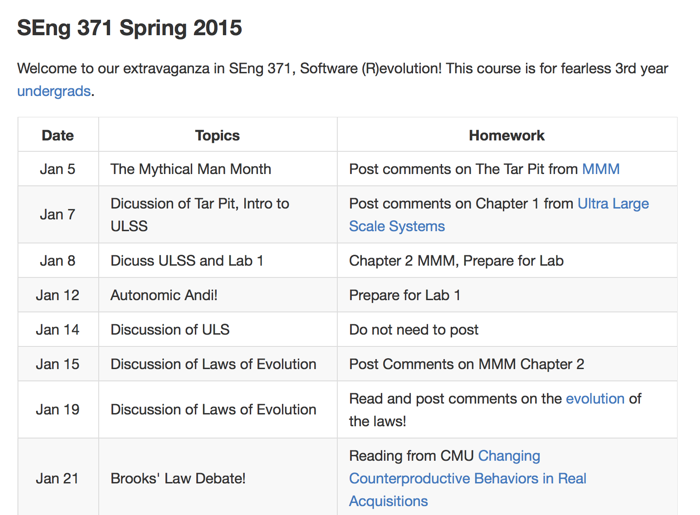
\includegraphics[width=0.8\textwidth]{schedule}
 \label{fig:schedule}
\end{figure}

The main use of GitHub was for material dissemination: the professor hosted a repository which all students could access to find the work they had to do for any given week. The instructor would update this repository weekly, adding lab assignments, links to readings, and the student homework for the week, as seen in Figure \ref{fig:schedule}. All of the content was organized into a calendar table made from Markdown, and it was visible on the home page of the course repository as a `readme' file.

The other main use case was in the repository's `issues' page, where all labs (2-3 hour long sessions once a week in addition to the course lectures) were hosted. These labs would often involve researching a topic and reporting results, or giving other groups feedback on their projects. A dedicated issue would be created for each lab, similar to a forum post, and students would then make comments on these issues based on their lab work.
%Lab assignments, however, were somewhat different between the two courses, where for Course #2 (Distributed Systems), labs tended to have more complex instructions

GitHub was also used for project hosting. Although students were not mandated to use GitHub for their course projects, most projects were hosted on GitHub in individual repositories. These repositories were public so others in the course (and outside, in some cases) could view the work and give feedback. %listed on Coursespaces

\section{Findings}

In this section, I present the findings according to each of the research questions posed for this study. For each question, I discuss the main themes that emerged from my analysis, providing relevant participant quotes from the interviews.

%The research findings are presented according to their related research question. From the analysis of the data, I extracted several common patterns in the participants' responses and categorized them into themes. Each theme will be discussed in detail and then accompanied by related quotes from the interviews as well as a list of participants that support the theme.

%Beyond the themes, some interviewees gave unique feedback that were not mentioned by others, but were noteworthy for several reasons - for example, they might speak to the potential of the tool or are unique drawbacks that only few people experienced. These will be highlighted appropriately and reasons will be given for why they are noteworthy answers.

%table of themes?

\subsection{RQ1: What are computer science and software engineering student perceptions on the benefits of using GitHub for their courses?}
In this section, I discuss the benefits that emerged from the students' perspectives from the three main uses of GitHub in their courses: for schedule and material dissemination, for discussions, and for hosting their project work. \\ %Many of these benefits stem from GitHub being a tool commonly used in industry, as well as from the advantages that Git offers for managing individual and group work. \\

\textbf{Benefit: Gaining Experience with an Industrially Relevant Tool} \\
In the current software development landscape, GitHub is a very popular tool for working collaboratively. As such, it is essential that developers are familiar with either GitHub or other distributed version control systems, particularly when working on collaborative, multi-person projects.

Students came into the course with varying degrees of experience with GitHub, as shown on Table \ref{table:interviews:students}. Five interviewees had minimal or no experience using it, while others were very knowledgeable about the tool, either through their own uses, through group projects for other classes, or through co-op jobs. Many, at least those who attended the University of Victoria for the majority of their undergraduate studies, had some experience with Subversion, a different version control tool that is taught in a second-year course.

Many of the interviewees mentioned that the use of GitHub in class provided a good introduction to the tool for them: \textit{``I think it's pretty good. I mean one thing is that because I'm using it in class, it's made me learn the tool \ldots and that's where the big takeaway is: that I've been able to transfer those skills, I've done some other projects just on my own time using GitHub.''} [P3]

%Others felt that in general, it was a good way of learning that way of working, which is beneficial for their careers: \textit{``I think [learning about the tool will] be very useful. Especially if I wanna work with any, open source, any newer companies, a lot of them have a lot of open source projects. Just knowing about version control and stuff like that is gonna be \ldots really useful in the future.''} [SE4]

For the most part, students who supported this theme believed that the use of GitHub for their courses and projects helped them experience a style of collaboration that they will encounter often in their careers. In comparison to the use of more traditional LMSs, one student noted why using GitHub might be advantageous for them: \textit{``Well, I like how it's like the extra bonus of more practice of something you're gonna use in industry, whereas none of us are gonna use Coursespaces or Connex when we're out on a co-op or out on a job.''} [SE3]

As well, putting their projects on GitHub provides practice for real-life scenarios. SE8 describes why it was beneficial to have their work publicly available for both classmates and outsiders to see: \textit{``I think when you go and work in software development too, you should get used to [having] lots of eyes being all over your work; that's just the way it's gonna be, so it's practice before real life.''} [SE8]

Beyond the benefit of using GitHub in programming projects, which is what it was designed for, the basic use of GitHub to manage course activities such as material dissemination and discussion was also beneficial to students as an introduction to the tool. \textit{``It's a good introduction to GitHub as a platform; it might not be a good introduction to Git as a tool. Because there's a lot of wizardry that you can do with Git that you'd never learn just doing what we did here \ldots but definitely a good start to get people using Git.''} [SE11]

Some students were introduced to specific GitHub features that they were not necessarily aware of. \textit{``This is the first time I've actually used the issues portion of GitHub \ldots So it showed me that portion of the capabilities of GitHub.''} [SE13]

Out of all the benefits described by students, the benefit of getting an introduction to GitHub and its features was talked about the most, as [SE2, SE3, SE4, SE5, SE6, SE7, SE8, SE11, SE13, DS4] specifically mentioned this benefit. The importance of this benefit is further emphasized by these students asserting their intention to continue using GitHub or to use GitHub even more after the course ends. This benefit was shared by students irrespective of their prior experience with GitHub. \\

%Those who had little experience with using Git and GitHub were given an introduction to the features of the tool and how `The GitHub Way' works, particularly when they used it for their group projects. Others familiar with using Git and GitHub cited others in the class or in their groups that initially weren't familiar with it and acknowledged the way in which the class allowed them to experience this tool that many felt was important to know about as a software developer or as a computer scientist.

%\textit{``Well I think the first thing is not quite everybody had used Git before. So for some people it was a bit of an introduction to it, but I think that's definitely a good thing. Better now than going on a coop, and the first day being like, \'here, here\'s the git repo'.''} [SE3]

% All of the interviewees asserted that they would use GitHub outside the class, whether or not they've had experience with it beforehand. \textit{``I've actually used it more now that since I've started using it in class actually.''} [SE2]

% \todo{candidate for cutting}
% \textbf{Benefit: Using GitHub as Storage} \\
% As an extension to this, many believed that GitHub use in the course benefited them in two primary ways. First, for those who were yet to be acquainted with GitHub, this introduction allowed them to experience its features and benefits, with many of these students asserting their intention to use GitHub more after the course is over. As well, for every student who would use GitHub to host and manage their projects in the course, many enjoyed the fact that their completed projects would be on their GitHub account publicly viewable for anyone to see. When asked about the motivations behind putting their work on GitHub, P8 explains: \textit{``to actually show to people and maybe have some people collaborating or maybe have employers see that I have worked on stuff \ldots I have heard about some of my other friends, like their interviewers actually ask them to look into their repos and they actually download it and install the software and they would talk about it.''} [DS4]

% One student believed it to be an useful tool for storage from the beginning: \textit{``I think it would have been great to have, especially in first year, if you did open one and use it throughout your education, it really does provide a place where all of your stuff is stored. You'll be glad that you can go back to all your old work.''} [DS3]

\textbf{Benefit: GitHub as a Portfolio} \\
Many students believed that using GitHub to host their course projects will be beneficial to them in the future. These students described that hosting their code from other courses or from personal projects on their GitHub accounts benefited them in various ways. For example, SE5 organized their code on GitHub for easy access when helping friends: \textit{``I know that when you're trying to help somebody out, you can always just say `Check out my GitHub', I know I've done that with a few of my buddies \ldots and I don't have to search through my files, it's just on GitHub, and you look on there. It's a good organization tool.''}

Many interviewees shared that GitHub could serve as a type of portfolio where their publicly-hosted projects and code could be used to present to potential employers when job hunting. Many employers nowadays refer to GitHub for hiring purposes\footnote{\url{http://www.cnet.com/news/forget-linkedin-companies-turn-to-github-to-find-tech-talent/}}. In fact, some of the students already experienced job interviewers asking them to show their GitHub accounts: \textit{``I think all three companies that I applied to this semester wanted me to link to my GitHub. So I was really lucky that I had [a class] project on there. And I think when this [course's] project is done too, it'll also be really nice to have up there, after we clean it up.''} [SE6]

DS2 also shared that interviewers inspected their code during an interview, highlighting the importance of having functional code in one's GitHub account: \textit{``These days I see that employers also want to see your GitHub page. While I was giving an interview for my coop, he did actually go into my GitHub profile and try to compile some of my code, so they do want you to have some online presence on GitHub.''}
%\todo{You seem to have repeated what you said above and not added anything beneficial. Rewrite or remove.}

%\textit{``Well I believe it's good for future employers. I remember I put directly on my resume saying you can check out the work I've done on GH. I included the link right on there and every person I handed my resume to were just like \'hey, fantastic!\' \ldots it's a good way to get your skillset out there.''} [SE5]

%The ability for students to use GitHub as a portfolio where they can show off their projects to potential employers was, for many, an important benefit of using the tool. There were students who were introduced to GitHub as part of their course, but knew the importance of having work on GitHub. This benefit motivated some students to continue putting their work on GitHub.
The benefit of using GitHub as a portfolio was shared by [SE5, SE6, SE7, SE8, SE11, SE13, DS3, DS4]. \\

%For others, having their projects from these courses hosted on GitHub could serve to benefit them for seeking employment in the future.\todo{this is a repeat of the intro to the paragraph}

\textbf{Benefit: Supporting Student Contributions to Course Content} \\
In the previous chapter, one of the benefits that GitHub offered over traditional Learning Management Systems is the ability for students to make changes, fixes, or suggestions to the course materials. Traditionally, this could be done by speaking to the instructor, either in person or by email, and then the instructor could make the changes as necessary. With GitHub, however, the students are able to make pull requests (PRs), changing the material themselves, notifying the instructor and prompting them to `accept' or `close' (reject) their PR as deemed appropriate.

Throughout the two courses in this case study, three PRs were submitted to make fixes to the materials or to add links to new materials. These pull requests were submitted in the first month of the courses and by only one student who was well-versed in GitHub (and who was registered in both courses). SE1 explains their reasoning: \textit{``I like being able to fix the mistakes that she might make like with a bad link or something by making a PR \ldots I really like being able to do that because you know, it makes me feel a little more involved.''}

This style of contribution didn't continue, however, perhaps because these initial pull requests to fix material or add links to other content were not merged quickly enough by the instructor and no one else was able to help. Another student described how this hindered more participation of this kind: \textit{``Because we did not have the access. If we had the access, then I think people would have collaborated \ldots I feel that either we should have had the access to merge it, or at least someone else would have had [access] who would have merged it quite quickly, like someone handling the pull request \ldots [Otherwise] that just defeats the purpose.''} [DS2]

Although SE6 did not contribute in this manner, they saw the potential advantages of using pull requests as follows: \textit{``I think everybody's had experience with mistakes in the course material. \ldots The alternative is just emailing the prof and asking them to change something \ldots this is always there, and they can always check it to see if there's something. This way someone can actually make the change, all they'd have to do is accept it.''} SE6 discussed the convenience this feature offers to professors, as changes are listed on a separate page in the GitHub repository and can be accepted with one click.
%\todo{why is this profound? it doesn't seem to offer anything.}

Of the three PRs submitted to the courses, two other students participated by either trying to accept the PR (and failing), or adding a `+1' to the PR's comments, supporting its acceptance. The following students agreed that being able to contribute to course materials via GitHub is a benefit: [SE1, SE3, SE5, SE6, SE10, SE13, DS2, DS4]. \\ %The benefit seems to stem from the fact that the process is straightforward (the instructor only has to accept or reject the PR) and it gives students agency in making these changes.

% As such, some believed the professor should have given indication that this was an option. \textit{``I think [the idea is] good, but I think it would've needed to have been advertised more that she was looking for input on things, and if she said that, maybe more people would have [contributed] to maybe propose like extensions for assignments or something.''} [SE7]

\textbf{Benefit: Support for Students to Contribute to Each Other's Work} \\
In these courses, projects were open and visible to other students, which allowed more opportunities for student contribution. This was demonstrated by a student's group working with others:
\textit{``For instance, one [issue] was our script wasn't taking in command line arguments if there were spaces in them properly. And then someone was like, you can just put in quotes. And we were like `oh, that's a lot better than what we were doing.' And then to be able to see what other people are having problems with and give suggestions. Even at one point, they were trying to find refactorings, and we said `hey you can use our tool, it'll help.' ''} [SE3]

Making students host their course projects on GitHub and relying heavily on GitHub in the courses resulted in students looking at each other's work (mandatory or voluntary) and making contributions in the way of advice or suggestions.\todo{I thought students didn't have to host their projects on github?} As well, students would actually utilize code from other groups and help fix issues in the code when necessary. \textit{``I believe that one other group decided for project 2 to use [our project 1] and they made a couple of pull requests I think.''} [SE10]

\begin{figure}[h!]
 \caption{A student providing feedback for other students' projects in an `issue'.}
 \centering
   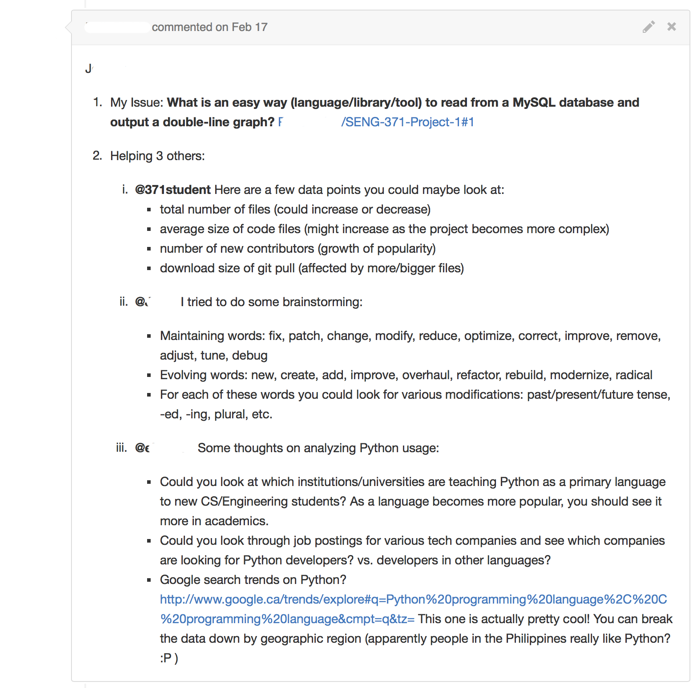
\includegraphics[width=0.9\textwidth]{contributing}
 \label{fig:contributing}
\end{figure}

Two specific lab assignments asked students to look at the repositories of other groups and comment on them, an exercise that students found useful, or at the very least, interesting. For students who spoke in detail about this benefit, they enjoyed receiving comments from the others: \textit{``Yeah, I liked getting the comments, I liked knowing that people were kind of checking it out, and I assume they would let me know if I was doing anything horribly wrong, and I didn't get any of those comments, I'm assuming that everything was going alright.''} [SE5] An example of a student providing feedback can be seen in Figure \ref{fig:contributing}, where a student attempted to give three other students helpful advice on their projects.

SE11 extended the concept of providing feedback to the idea of peer reviewing, where students would judge the work of others and make comments on their work. SE11 explained the benefit of having others looking at and judging their work: \textit{``I thought [peer reviews] was the best way to learn actually \ldots It forced you to put yourself in a position where you have to defend what you did, which I think is good for quality because you have to actually care.''}

Helping other projects, either through discussion or through collaborating on the code, offered students new ways to participate that are unique to GitHub and similar types of systems. Students effectively collaborated with each other with the aim of producing better work, as was noted by [SE2, SE3, SE5, SE7, SE10, SE11, SE12, SE13]. \\

%Discussions were another way that students felt was a good way of participating in the course. Although discussions are a part of multiple other tools, GitHub's discussions, via the Issues feature, provided an advantage that others didn't - Mentions. By typing someone's username preceded by the \'@\' symbol, the user gets \'mentioned\', and this has two implications: a) other users reading the comment know who the comment was addressed to and b) notify the user being mentioned that someone mentioned them in a comment.

%In the Issues for the classes (which acted as the Labs), many students would use it simply to sign their work or acknowledge their group members as part of their answers. However, during labs where interactions were more encouraged, such as when they were set to comment on each others' work, students would use this Mentions feature, which would notify those mentioned that a comment was directed at them. Some found this useful: \textit{``I really like how once somebody's commented on the thread, you can just use the little @ symbol and send them a notification and vice versa. When someone mentions you in a comment, you'll see it on your email. Which is good.''} [SE2]

% \todo{Getting Inspiration from Each Other's Work?}
% \textbf{Benefit: Getting Inspiration from Each Other's Work} \\
%seeing other groups work
% As described above, the open and public nature of how GitHub was utilized in these courses meant that students could easily see each other's projects. Though most only looked at other group's projects when mandated by a lab assignment, some interviewees found this aspect of group work helpful: \textit{``It's nice seeing what everyone else is working on, because you're working on your own project, and you kind of get into your own little world, and then.. Yeah it's really interesting to see the other creative ideas that other people come up with \ldots I actually think there was one person on [another] group, they had a really really interesting question, I kind of followed their repo as they went along, and finally got answer.''} [SE5]

%Some, however, found this exercise only potentially helpful:
%\textit{``I think that it could be useful, I mean for my project, I definitely read through the other comments. But I already like a pretty good idea of what I thought I was gonna do, so I definitely took some of them into consideration, but I wouldn't say it was like super valuable for me, personally. But maybe if you like, if you actually were having big issues with your projects, and you don't know where to start, it might be useful.''} [SE2]

% While others took little time to go through other groups' repositories beyond what was required for the lab. When asked why, SE6 responds: \textit{``Maybe [I'll look at the other repositories] at the end of the course. But like I know what ours looks like right now \ldots It's a work in progress and I assume other people's are the same right now.''} [SE6]

% Some, however, took little time to go through other groups' repositories beyond what was required for the lab assignments, often because of time issues: \textit{``I think it is important [to be able to see other people's projects and give feedback] and it's neat that it's all out in the open \ldots the other thing is there's just so much going on with all the courses that it's hard to pay attention to every other project, and even get remotely invested in them, because it's almost a challenge to make sure yours is working.''} [SE10]
%
% For the lab assignments, every student would post something that was visible to the rest of the class as a response to the week's lab topic. Many students discussed the benefits of having this type of submitted work available publicly. Students found value in being able to see the work done by others for reasons such as comparing their work, learning from others, and even just curiosity.

% \textit{``The one nice thing I like about just being able to do the issues like this as opposed to like a regular assignment submission is that you can see what the other people are doing. Which is really helpful if you're a certain standard of how much everyone else is typing, as well as if you're just out of ideas and you need somewhere to start with you're like, alright, that's an interesting idea, maybe I could look at that a little bit more.''} [SE2]

% \textit{``It's nice being able to see everyone else's answers, it's not just you writing an assignment and you handing it in and you don't really know what anybody else has done. And the questions have been constructed in a way [such as] \'find three tools\', so it's nice being able to review the tools other people have found, because you might not have found them either.''} [SE5]

% It should be noted, however, that this style of lab assignment submission is easily replicated in traditional LMS through the use of forums and discussion boards.

\textbf{Benefit: Keeping Each Other Accountable} \\
One benefit that stemmed from GitHub's transparency features was the ability to see a history of commits to a project. This was cited by some students who used GitHub to manage their group projects---they could easily see if and when their partners submitted work. Their repositories kept an account of when each change was made, which provided collaborators an easy way to track the work being done on the project. This helped the students to keep up with each other's work: \textit{``You can see exactly what the other person has contributed, and you can look it up again a month later \ldots So then if they're trying to say that `I did this huge massive thing', and you look and it's only like teeny-tiny, then it's a good way to keep accountable. And it's good for yourself too, because you know they can see your work, so you wanna make sure that it's top notch and easily readable.''} [SE5]

%\textit{``And just being able to see what other people are doing on the repo you're working in, is kind of a motivation in a way too. It's like, oh hey they're working on this, I wanna do something cool like that too.''} [SE3]

Moreover, the students knew exactly how much work each member of their group contributed to the project and this helped the student keep themselves and each other accountable: \textit{``We decided to switch to pull requests instead of just committing straight to master, because \ldots for a couple of reasons, first of all, if there's something like majorly wrong with it, everyone can see it, right? And the second thing is, everyone sees it, so if people have to work on [the same code], in the future, which we all did, then they know exactly what just went in, so that next time they come to the code and pull it, they're not like `where did this all come from?' ''} [SE9]

This is a useful feature to have when working in group work as it allows for awareness between group members. By using GitHub for their group projects, students were able to take advantage of the collaborative features that GitHub offers to improve their processes or their product. This benefit was described by [SE5, SE9, SE11]. \\

%add SE3 quote here from slide 16

%professors too?


%able to see when repo is updated
%Having the course materials and schedule on the GitHub repository was helpful to some students thanks to the Transparency features of GitHub. If a change has been made or if the professor added something new to the repository, they would be informed in their News Feed and, if they are subscribed to the repository, by an email sent to them.

%\textit{``I think once you star something, you get notified for every push to master, so you get all the changes to like, this home page readme, and anytime a new issue is posted.''} [SE7]

%Unfortunately, some experienced issues with this, particularly when they were subscribed to the repository. This will be covered later when their responses pertaining to Research Question 2 are highlighted. As well, only a few students cited this as a benefit, with some not even knowing that it was possible to get notifications by watching the repository and describing that as a weakness of the system.

\textbf{Benefit: Version Controlled Assignments} \\
Using version control for their assignments and projects benefited the students in multiple ways. DS1 worked alone on a project and shared that using GitHub \textit{``makes it more traceable \ldots you can see when and where [your work has been done].''} This student utilized the history of their commits as a reminder of where to continue from when they returned to work on their project. For others, the ability to revert to previous states of the code was useful: \textit{``You're working on a project, and you make a change that breaks everything. Well you can just go back to a different commit, one that works. Boom, fixed, try again.''} [SE11]

Although the instructors for these courses did not use their repositories for marking, some students believed the system could allow instructors to give constructive feedback as they built their projects and assignments. One student believed that the ability to see the student's process could be important: \textit{``You'd see all the mistakes they made getting there, too, which is just as important to learning as the finished product.''} [DS3]

SE8 described a hypothetical situation where professors could use the student's repositories as submissions as opposed to the traditional way of submitting through an LMS: sending the code only when finished. SE8 said that this way of submission would be \textit{``so much more useful \ldots You could see everybody's contributions, you could comment on them too \ldots Unless you're doing a live code demo with a TA or any instructor, you're not getting any real feedback [with the traditional submission system] \ldots You have no idea where you lost the marks or where you went wrong.''}

Students felt that hosting work on GitHub and using Git to manage their work was beneficial because of the ability to pull from anywhere, and to see and be able to revert to previous versions. As well, they believed that having instructors use version control to mark their work could be beneficial (if implemented) because of the new ways in which they could provide feedback. [SE1, SE2, SE8, SE11, DS3] shared this benefit. \\

% Though not necessarily related to how GitHub was used in their class, many students described advantages to using GitHub to host their school work, including their projects for this class. For one, students enjoyed being able to do their course work from any computer. Some students who were more experienced with using GitHub claimed they would use it for all of their course work for this very reason. \textit{``And that's sort of where we're at, it's like I use it for everything. Even when there's no specific mandate for it, just the ability to pull it down in multiple places is worth having.''} [DS3]

% \textit{``For me, the reason I started using it is because you know, I would start working on a project at home, and then realize 15 minutes into it that this was my saved version from a week ago, and I had done work since. Like \'oh it\'s on the school computer I need to go get it'. [And then] it finally clicked \ldots I think it's really beneficial, by the time you get to 3rd year, for like networks, the big multi-week coding assignments that it\'d be really useful for.''} [SE6]

%version control, potential feedback. p7, group

\textbf{Benefit: Connecting with the Outside} \\
The final benefit that emerged from the interviews relates to the way in which work hosted on GitHub is often publicly available for others to contribute to. For example, SE1 was highly active in the community of a certain programming language, and for their first project, they were building something related to the language. They advertised their work to the community, and members from the community then tried to help with their project in multiple ways: \textit{``So here I have people involved in the discussion. These are just people in the community I've been talking to about how to do different things, and they've been giving me suggestions. And that's really cool because I actually have like some community involvement in my course project.''} They also noted how this was helpful: \textit{``But for me, I find it really validating when someone else is like `that is really cool, have you considered doing this?' ''} [SE1]

SE1 was the only student interviewed who used the public nature of the course projects to solicit outside contributions. However, the exposure to GitHub gave students opportunities to discover work outside of the course and to use other repositories to aid their projects. When prompted, most interviewees mentioned that they sought out public repositories either to pull their code and use it, or to find inspiration for their own projects. One student recalled an experience where their group looked at an open-source library: \textit{``We just looked at how Gitstats, [an open-source library] did it, and then wrote our own thing into our project \ldots I think that more than anything is the biggest reason why Git should be used for education, because it takes, I think, until you start being forced to do it \ldots to actually go and look at other people's code, and I think looking at other people's code is like the most important thing.''} [SE6]

Speculatively, however, this likely would have happened regardless of whether or not GitHub was pushed by the professor as students tended to seek out other code and libraries for their projects: \textit{``And in industry, the first thing you do is check Stack Overflow, look for someone else who has done the same thing and jack their code.''} [SE7] [SE1, SE2, SE3, SE4, SE6, SE7, SE10, SE12, SE13, DS2, DS5] mentioned looking at outside work and public repositories for their projects.

\subsection{RQ2: Will students face challenges related to the use of GitHub in their courses? If so, what are these challenges?}
This section outlines the challenges the students described relating to GitHub use in courses. Some of these challenges were related to tool literacy, where more knowledge of the tool and more experience using it in an educational context could have mitigated the challenges. Yet, they are worth mentioning as potential challenges that students might encounter. \\

\textbf{Challenge: Privacy is All-or-Nothing} \\
While hosting student projects on GitHub publicly provided several benefits, others acknowledged the potential issues that follow: it may not be appropriate for a class environment. SE4 describes this dilemma: \textit{``So [using GitHub for your work has] got benefits and drawbacks: benefits being that other people can access your data, drawbacks being that other people can access your data.''}

Most interviewees didn't mind that the class repository and their project work was public. However, many students could see the potential problems that might surface from their work being publicly available. Students mentioned that although they would ideally put 100\% effort into all their submissions, this is not always realistic due to the time constraints students face. For example, DS3 noted that although it can be advantageous to host code publicly so that employers are able to see their projects, the employer may not always agree: \textit{``I think it comes back to what do you want to show your employers? When your employer looks at your work, will they understand that work I submitted in Git was when I didn't understand yet what I was doing, I was still learning? \ldots If I could make the assumption that an employer would understand that, I would have no problem with it being public. That said, I can't make that assumption. I have to assume that everything they look at they're judging in the harshest light possible. So I try to show only things that are of quality that I'm proud of. And that's unfortunately not a lot of the classwork until I'm done with it and the final product I'm happy to show, but all those steps getting there, they're often filled with pitfalls and horrible programming and badly factored code.''} As such, courses mandating the use of Git and GitHub to publicly host student work could be problematic for students if employers are looking at work-in-progress in a negative light.

%not everything is 100% effort
SE6 acknowledged that sometimes, students rush through their work, and therefore, they might not want that work to be publicly available. \textit{``You know it would actually be nice if they were separate or private somehow so I wouldn't have to go through everything and sanitize all the stuff I've submitted, because you know, for as much as you'd want to think you're putting 100\% into it, you're not really, you know, writing some great work of art or careful analysis, so private would be nicer. For things like that.''}

%not everything is of interest to public
As well, SE1 felt that some of the work in the course repository wouldn't even be of interest to the public or to potential employers, and as such, they saw no need for the repository to be public: \textit{``I'd rather have [our comments] be private. But only because there's not a whole lot of participation, so I don't feel they're of interest to someone publicly.''}

% \textit{``It's good for finished projects, but not all that in-between stuff. I don't wanna show these issue things that I've submitted, to employers because they'd have to wade through that. They don't wanna see that, they wanna see finished projects and what that looks like after you're done.''} [SE6]

Yet, others saw no issue, and even preferred all their work to be in the public space. \textit{``Personally I don't have a problem with it being public. I would like to have a good online activity of myself on GitHub, so that's not really an issue. I'm not really concerned if someone is going to read my blog or not.''} [DS2]

There are workarounds to some of these privacy issues, where students do not have to attach their names to the work they contribute to the GitHub repositories used for the courses. \textit{``I think part of that would be.. you can decide that on your own, depending on if you use like your main git account or just make like a separate git account for your class and whatnot.''} [SE3] Indeed, one student created a new GitHub account solely for contributions to the class. Unfortunately, this student did not want to be interviewed, and group members were uncertain as to what the motivation behind creating a new user was; presumably, they were motivated by some of the issues discussed above.

In summary, although students enjoyed the benefits that came with making their work publicly available, many students also acknowledged that these benefits are accompanied by a number of caveats. Importantly, some students described the lack of a middle ground as a limitation, where in the context of this course, students had to host their work publicly. This challenge may be mitigated by the instructor giving the students the option of creating a new GitHub user account for work done in their courses, as suggested by SE3 above. This challenge was shared by [SE1, SE4, SE5, SE6, SE7, SE10, SE13, DS3, DS6], while [SE3, DS2, DS5] disagreed that there are limitations to publicly hosted work. \\

%first group's submissions rule all
% A benefit cited earlier was the openness of the tool, where students are able to see each other's work and submissions to the lab assignments. However, many acknowledged that this way of working where everybody in the class can see submissions simply could not work in other types of courses, particularly those in which assignments have only one solution. \textit{``In this particular course, because each person's project is so different and unique, there's really no way you could do plagiarism, it just doesn't make sense. But if for some courses where everybody is giving the same exact assignment, and you're all on GH, I think I'd be a little more nervous about putting my code up. ''} [SE2] This is further discussed in RQ3.

% In fact, some saw this effect even on the lab submissions in this course, even though lab work typically varies from group to group. \textit{``I'm not sure if it's good or not that we can see other people's submissions as we go along in the lab. Because I think, because of that, all of the submissions have ended up looking like the first submission.''} [SE6] However, as mentioned by many students, this is potentially a benefit, by giving them examples to follow or a standard to measure up to.

\textbf{Challenge: Lack of Training on Git and GitHub} \\
Another issue that many students described related to education and training---there were varying degrees of experience with and knowledge of GitHub and its features, which presented difficulties with the use of GitHub in these courses. For example, SE9 believed that students who were less experienced with the tool could not take advantage of its benefits, such as the ability to make pull requests on the course materials. SE9 believed that if the professor did not set a precedent for that behavior, it may not be used: \textit{``I think you just have to, 1. advertise it so that the students know [to] use this as a communication tool. And then 2., kind of layout, or give some examples on how it could be used.''}

This lends itself to a bigger issue---educating students on Git and GitHub's features and on the instructor's intended workflow for using the tool in the classroom. The main course instructor for these two cases inexperienced with using GitHub, which made it difficult to educate the students on its features and caused some frustration for some of the interviewees. In fact, most students who were asked mentioned that the course could have benefited from more education on Git, GitHub, and what they can do with it. Students said that they could have hosted a lecture or a lab dedicated to learning the tool, perhaps at the beginning of the course or as an extra session. \textit{``I think it would've been good to do some demo \ldots cause I think [the instructor] talked too much about theory in class and there's no actual coding or no actual demoing.''} [DS1]

%\textit{``I wish [the instructor] knew how to use GH, that would be nice. Because yeah I was submitting pull requests to actually make her readmes that were .markdowns markdown files instead of html files, and stuff like that. ''} [SE1]

%Those experienced with GitHub still acknowledged the usefulness of hosting such a session: \textit{``there's people who have never used it, like [a group member] in our group has never used it so she's just getting used to all the features \ldots if we wanted to maybe tie it all together, it probably would've been useful to have a little Git session for the people who didn't know how to use Git''} [SE6]

%\textit{``Even just like on the first day of the lab just going through some of this stuff. I think what we did on the first day was that if you didn't have a GH account, you were supposed to go and create one. That part's really straightforward, commenting on issues is really straightforward, that's no problem. The only problem is when you actually start working with code and working with versioning...''} [P3]

SE2 acknowledged the potential difficulties in hosting such a session: \textit{``On the other hand, when someone teaches it to you, it often doesn't make sense until you actually do it yourself. Cause you'd actually have to go through the struggles of actually doing a commit and like pressing all the buttons, so I don't really know how much could be done in that regard.''}

Students also asserted that the University of Victoria needs to further emphasize teaching version control systems such as GitHub in the undergraduate level. As it stands, there is one required course that students said that teaches version control systems and how to use them, utilizing Subversion and touching on Git. Some students, however, felt that one course was not enough, particularly when Subversion is much less popular today. \textit{``I think in [SENG265], we did SVN, which is a good introduction to the idea. But I don't think it's widely used anymore.''} [SE3]

% \textit{``, I could tell you I think it was SENG 265. And it was, we were kind of introduced, we were told what version control was, and \'oh yeah you could use SVN or you could use Git, or both\'. We were kind of introduced to it, we were never required, or even really pushed to use it''} [SE5]

% Some would lament the theoretical focus they believed the undergraduate software engineering or computer science departments had: \textit{``I think that's one of the biggest problems, even SENG being taught in a university that focuses a lot on theory, and not a lot on technical.. like one of our only classes where we got to actually learn technical skills, and it's a really technical area.''} [SE8]

Three of the interviewees, [SE1, SE6, and DS3] believed that students should get an account quickly after their first introductory Computer Science courses. \textit{``if I was teaching someone how to code, as soon as they start working on code that was bigger than 100 lines, I would teach them how to use version control.''} [SE1]

% \textit{``The first class where you have a big project, like a group project where you're sharing code, it should be taught''} [SE6]

%However, DS5 believed it is important to communicate the benefits of using such a system: \textit{``The first challenge is to get them really interested, because many of them are exposed to many other tools already. So I think to really bring up the advantages [that] GitHub can bring to the students so they can use GitHub as a primary tool and convince them that it's really good''} [DS5]

This issue is related to tool literacy, where an instructor who is experienced in using GitHub might have been able to better educate their students on GitHub and the features they intended to use. Beyond the instructor, this issue could have been alleviated by a greater focus on version control and DVCSs and what students can do with these tools earlier in the curriculum. As it stands, students were not able to properly utilize some of the benefits of using GitHub due to inexperience and unfamiliarity. This was discussed by [SE1, SE2, SE3, SE4, SE5, SE6, SE9, SE11, SE12, SE13, DS1, DS3, DS5]. \\

\textbf{Challenge: Notification Overload} \\
Although few students brought up this issue, how GitHub handles notifications from the repository emerged as a challenge. The only way to get notifications from a course repository is to `watch' the repository. `Watching' provides two different options: 1) to get a notification and an email only when the user is mentioned in issues or commits, and in discussions the user has commented on, or 2) to get a notification and an email when anything at all happens in the main branch (master), when someone comments on issues, commits, or pull requests, and when someone makes or accepts a pull request. The `watch' feature comes with some drawbacks, not the least of which was when a student was not very familiar with this feature and therefore did not use it: \textit{``I didn't like that [repository] at all, because I didn't get notified when she adds stuff to there, so I don't really know what's going on without remembering to check it on GitHub. ''} [SE9] This student did hear about the `watch' solution, but thought that it \textit{``would be a good solution, but it might be overkill. For like a spelling change.''} [SE9]

Unless students were `watching' the repository, they would not receive email notifications for any activities unless they were directly mentioned. However, if the students did `watch' the repository, they would receive an influx of notifications for every user comment on the discussions, which can overwhelm the student. SE10 shared that they were engaged less in the activities of others because of the noise from notifications: \textit{``It sent me a million emails, both of [the tools] actually. I should have just turned that off, but I was worried about missing something. Because everytime someone would post, you would get another email \ldots I actually did not read anyone else's feedback because it was just so many emails, to be totally honest.''} [SE10]

As such, the `watch' feature was problematic for courses like the ones studied, where every single comment would trigger a notification and an email, causing an overload of notifications. [SE7, SE9, SE10, SE11] shared this issue.

%- Integration with UVic
%Another point that students felt would hinder GitHub as a learning tool was the lack of integration with the University of Victoria login, similar to that which LMS such as CourseSpaces have. This means that students will have to create new accounts to an external site (if they didn't have one already) and, more importantly, that the administrative tasks that LMS usually take care of such as grades and class participant lists cannot be done on a tool like GitHub.

%Hmm.. The one thing about CS is that it's all integrated with the current school system. So in terms of like adding your grades and feedback that way, I don't think profs are even allowed to upload grades into GH, there'd be some big issues there. *laughs*. So.. that'd be one thing. [P3]

%Uh, it's fine, but we like to, we like to get a more into interactive with the CS. For example, if somebody post something on GH, we couldn't know anything that is not on CS, because these two are not connected. [P9]

%Right now I have to say GH is... to me, I value them equivalently, just because the university enforce CS into their system. So I'm pretty sure in the future if the university can include GitHub into their university system, I think students are more prefer GH. [P9]

%Uh, the only thing I can think of is maybe somehow.. I don't even know how it would work, but if they could somehow be.. connected with UVic. Like, I'm not even sure how that would work, but.. some sort of academic affiliation or something. [P10]


\subsection{RQ3: What are student recommendations for instructors wishing to use GitHub in a course?}

Given that the use of GitHub in these courses was relatively basic, many students, particularly those who were experienced with using GitHub for collaboration purposes, had ideas on how GitHub could be further utilized to be more beneficial for both themselves and for their professors. Many students discussed recommendations such as which classes GitHub could best serve and the need to utilize additional GitHub features. This section outlines those responses, highlighting the suggestions students gave about the workflow for using GitHub in a course. \\

\textbf{Recommendation: Use GitHub in More Open-Ended Courses} \\
As discussed earlier, students had concerns regarding the public nature of the work they host on GitHub. While most students interviewed did not mind their work and their comments being in the public space, there were concerns regarding how this way of working could apply to different types of courses, particularly courses in which students are afforded less freedom in the nature of their work. %As well, some did not even see sense in keeping a course repository open for the public because of issues highlighted earlier, such as that it just won't be interesting for outsiders and that their work might often be rushed and therefore unappealing to have on display.

As such, some students [SE1, SE5, SE6] suggested that for courses where the discussions are self-contained, the repository does not need to be public. This would avoid some challenges, such as students submitting incomplete or messy work, but would also conflict with some of the benefits extracted from these interviews, where students can build their online presence with public work and instructors can make their course open for outsiders to contribute to. A suggestion for avoiding these issues came from one interviewee: \textit{``I think that as long as we have the option to make [our discussion comments] private, maybe after the course ends. So keep it intact while the course is ongoing and then we have the option [to change the privacy], everything will be okay.''} [SE12] Currently, GitHub does not support doing such tasks, unless the course instructor decides to privatize the course repository as a whole after a course ends, or an individual student deletes their comments and posts. %While this is a potential solution, these tools like GitHub would need work to meet such a solution. %this might be DSCS-worthy

However, students had opinions regarding what type of course would best suit GitHub. Interviewees suggested that a course similar to the two cases studied, where the work is very open-ended and could therefore exist in a public space, is where using a tool like GitHub would benefit the students most. When asked about their experiences with viewing others' projects in this course versus in other courses, SE7 said: \textit{``I would say this class is specifically different because we had so much flexibility over what we were doing. It's not like in our Operating Systems class, [where] it's like go make this shell that does this, this, and this. Where this was way more open ended, everyone's doing something different, so even if you could see what everyone else is doing, no one could've helped us.''} [SE7]

Students acknowledged that the open-ended nature of these courses was what enabled the successful use of GitHub, but that it would not work in less open-ended courses because of plaigarism concerns. Regarding the potential use of GitHub in their future courses, SE5 discussed: \textit{``Like I said, I like seeing other people's work and whatnot. Maybe not if everyone has the same assignment, because everyone's just gonna cheat off each other.''}

%\textit{``It works really well for this too, because it's not the same thing that everybody's submitting. So even if the format's the same, the content's gonna be different. So obviously if it was something where there was an answer, it'd be awful for it.''} [SE6]

% \textit{``With something like Operating Systems class, where everyone's building a shell, and it's all in C, you all have the same system calls and it's more like a puzzle where you gotta put it together the right way, you can just look at someone else's and be like `oh that's how that's done', right? \ldots If they have everyone's code up available to everybody, then that's kind of pointless.''} [SE7]

These students related back to the privacy issue, where having completely public work might be a detriment to the work being done when there are concerns of plagiarism, such as when the assignments posted have a single solution. Some students such as SE6 attempted to conceptualize a way to use private repositories, but ultimately felt it might be too cumbersome. As such, students believed that instructors would have to consider the nature of the work before deciding on the workflow they use GitHub with, or indeed, whether they want to use GitHub at all. This consideration was suggested by [SE2, SE5, SE6, SE7, SE13].

It should be noted that there are ways to use GitHub privately within a course, where even student assignments are private. This type of workflow involves the instructor creating an organization and having each student create private repositories for their work to keep them private from each other. However, this workflow would then minimize many of the benefits listed in RQ1. \\

% With no formal assignment submission feature, students believed that GitHub would struggle when students were uploading their assignments if all the assignments had a specific answer. SE6 brainstormed a potential workaround: \textit{``I was thinking you could even do that with like pull requests, you just start a PR, each person just a PR, and the teacher just accepts all of them on the due date, or whatever.''} [SE6] However, this is indeed a workaround and may require more effort from the parts of both the instructor and the student.

\textbf{Recommendation: Mandate the Use of GitHub's Collaborative Features} \\
The students who were more experienced with GitHub mentioned that GitHub's more collaborative features should have been further utilized to take advantage of the uniqueness of GitHub over traditional LMSs. One issue that some students discussed was that they saw little reason to use GitHub for courses if it was used only for material dissemination. For example, as mentioned in RQ1 above, only 3 pull requests were made throughout the semester.

DS3 was very outspoken on why using GitHub for this course was somewhat unnecessary: \textit{``I don't see any benefit that GitHub has offered that we wouldn't have had in CS. All it appears to me is it's a place where it's a file repo, \ldots and we already have that.''} They also noted that while there's potential, the unidirectional nature of the work being done meant that the potential benefits were not realized. \textit{``If there was a way to collaborate on the material, that would be useful \ldots But in this class, every one of our labs so far has been demo to the lab TA, so nothing's going back to GitHub \ldots Maybe if we were submitting things to it, maybe that would be helpful. I can see how it could be useful, it's just that in our usage it's not really adding anything to the experience.''} [DS3] It should be noted that this student's project group did not use GitHub to collaborate, but they used Docker Hub\footnote{\url{https://hub.docker.com/account/signup/}} instead.

SE7 echoed these sentiments: \textit{``I think that you can accomplish the same thing with a simple HTML website, honestly \ldots It's not using a lot of the features of Git, like looking at changes, commits, pull requests. The issues were kinda cool for the lab, and, again, you can accomplish that with any sort of forum, I would think \ldots We're not actually delivering code to the professor, so maybe it doesn't make a ton of sense [to be using GitHub].''}

As such, many students believed that GitHub was not being used to its full potential in their courses. The underlying suggestion was to consider which features of GitHub the instructor would like to use, such as pull requests or grading via commits, and use those features thoroughly and consistently. As it stands, some of the benefits they described to using such a system were only possibilities. An example which will be highlighted later in Section 5.8 was reported from a student in the DS course, where even the issues were not used for discussion during labs. \textit{``So basically we had to show it to our TA that we have done [the lab], and he used to mark it in a piece of paper. So putting [our responses in the issues] was not really necessary?''} [DS2]

An important lesson to learn is that GitHub only equips instructors and students with the possibility to take advantage of the benefits on offer. It is then up to the instructor to realize those benefits by using the features involved. [SE3, SE5, SE6, SE7, SE11, DS2, DS3, DS4, DS6] touched on this suggestion. \\

\textbf{Recommendation: Define and Advertise a Workflow} \\
Students acknowledged that GitHub was not being used to its full potential and that there was confusion surrounding the use of two tools (GitHub and Coursespaces). Coursespaces was used to fill some of the gaps in education support offered by GitHub, such as private forums and a gradebook. However, students tended to be displeased with this decision: \textit{``One thing I really don't like is that we have both systems set up, and so sometimes the announcements are in GitHub, and some of the times, they're in CourseSpaces, and that can get kind of confusing, like did she post an assignment here or here?''} [SE2]

This was an almost unanimous issue between the students interviewed, with only a few stating that they did not mind either way. Most mentioned that they would have preferred the use of just one tool, even if everything was public in GitHub. As a result, many students suggested that it would have been important to define a workflow for using this tool in a course in order to gain the benefits described earlier in the chapter. This workflow could include aforementioned activities such as utilizing pull requests or using just one tool instead of two. In the case of pull requests, for example, students advocated that the instructor should be advertising their use, thereby defining to the students that contributing to the material would be part of the course workflow: \textit{``I think [the idea is] good, but I think it would've needed to have been advertised more that she was looking for input on things, and if she said that, maybe more people would have [contributed] to maybe propose like extensions for assignments or something.''} [SE7]

One student mentioned that although GitHub does not do everything needed in a course, defining a workflow will cover up many of those weaknesses. \textit{``Even if there are no enhancements on GitHub, but if you define a proper workflow of using it, then it can be quite successful, because even the present Learning Management Systems are not perfect right?''} [DS2]

While most students did not have suggestions as to what workflow to use, they acknowledged the importance of defining it and teaching it to the students early on in the course. SE6 wanted to \textit{``enforce more actual Git and GitHub features in the way that we interact with the course material, and enforced GitHub use for actual projects. In a way that everybody had sort of a base level of understanding. So maybe at the beginning of the course \ldots there should definitely be a time when you learn Git.''}

In summary, many of the students interviewed were frustrated by the lack of a clearly defined workflow, and believed that the course would have been improved greatly if a workflow had been defined and advertised in the beginning. This recommendation emerged from interviews with [SE1, SE2, SE3, SE4, SE5, SE7, SE9, SE11, SE12, SE13, DS2, DS3, DS4, DS5].

% Beyond the workflow for the course as a whole, some also had difficulties getting on the same page as their group because there was no defined workflow. \textit{``I initially wanted to post all the issues and our conversation so we could account for who's doing what. But they basically didn't respond to them at all, so I moved to email. They responded to that a couple of days later so that was nice.''} [SE1] As such, students believed that having a properly defined workflow would go a long way towards reaping some of the benefits and bypassing some of the limitations behind using GitHub as a learning tool.

%doesn't belong here
% Other students would acknowledge this is a nice benefit of using GitHub in this manner, claiming that it's something they could see themselves using had they known that it was an option. When asked about changes to make with the course and its workflow, SE3 answers: \textit{``Like maybe if we can incorporate PRs in one way or another. Maybe with the idea I mentioned before, of having everyone contributing to the main repo \ldots That would be neat and beneficial.''} [SE3] %\textit{``So it's good that other people, like students can also contribute to it \ldots [it brings] more involvement from other people as well.''} [DS4]

%Uh, I would create students directories, one for each student for the course, they have their own directories. Later on, if there's group work or group projects, I would at least like students to form a group and create their own project directories in there. And they can view their stuff as well as outsiders can also view what's going on the course. [specific workflow]

%Yeah, I would like to see Yvonne maybe using the Wiki a bit more. Because the readme's good, but it's very long. So and the readme, I think should be more of a directory, like go here for this, go here for this, and key updates, like don't forget the midterm on Thursday. But the wiki you can actually construct it like a book. So that would be nice if that was set up. [workflow]

%I think more teaching on maybe more common industry practices when you go about it. Cause there's so many ways you can use GH, and I was actually looking at some other people in our class' GH pages, and the way they did it was quite different from the way we did it. Like we did the whole PR workflow, which, I don't think I'm biased but I think that's like a really good workflow. And then you see like other people aren't even using issues so.. I think maybe just a little more teaching on the capabilities of GH.


\subsection{RQ4: From the student perspective, how does GitHub compare to traditional Learning Management Systems?}
One of the goals of this research study was to discover the effectiveness of GitHub as a tool when used in ways similar to Learning Management Systems. Several instructors that we spoke to in Chapter 4 described using GitHub for purposes that LMSs typically serve. As discussed in Chapter 2, LMSs tend to be limited in that they encourage self-contained courses and focus on administrative and teaching features rather than on student activities. As such, the use of GitHub as an LMS is a use case worthy of investigation. The primary activities performed with traditional LMSs include material dissemination, evaluating students, and discussion among the students and instructors. Below, I discuss some of the comparisons students made through the interviews with them. \\

\textbf{Comparison: GitHub Lacks Threaded Discussions} \\
When GitHub was compared to traditional LMSs students have used at the University of Victoria (Connex/Sakai, Coursespaces/Moodle), many of our interviewees mentioned discussion and forum features. For both courses in this study, there were two main platforms where students could discuss and comment: on the course repository's GitHub `issues' page, and on Coursespaces' forums. The professor separated these by assigning all lab work and discussion to GitHub and the assignment readings and comments to Coursespaces.

Students were generally receptive to the use of issues as posts, particularly as it offered flexibility not seen on regular forums. For example, students liked the ability to `mention' others and to receive notifications when they are `mentioned', as they felt these notifications were convenient and efficient. \textit{``I really like how once somebody's commented on the thread, you can just use the little @ symbol and send them a notification and vice versa. When someone mentions you in a comment, you'll see it on your email. Which is good.''} [SE2] The `mention' feature is furthermore generally unavailable in the discussion features of Learning Management Systems used in the University of Victoria.

However, not all the students appreciated using GitHub Issues for discussions. The main difference between the `issues' page on GitHub and the forums in traditional LMSs is the lack of `tree-style' discussion in GitHub where all comments on an issue are arranged by time in a linear fashion. In the Coursespaces forums, in contrast, there are top-level comments in a thread which users can reply to individually, and these are arranged in a manner which makes conversations easy to follow. \textit{``GitHub unfortunately doesn't have any sort of like tree style view of conversation, it's just linear, so it's really hard to actually have a conversation between multiple people \ldots As opposed to Coursespaces, which is kind of more tree-styled.''} [SE1]

The main issue, according to SE1, is following these conversations: \textit{``And you literally have to go and search for all of the conversations from foo and bar and try to piece them together. It would be nice if it had like a reply that would put it right underneath.''} [SE1]

% Students who offered up suggestions for possible improvements to GitHub often discussed changes to this style of commenting, advocating a style similar to that of Coursespaces. \textit{``If there was a way to actually directly reply and keep track of what's going on, it would also be a lot easier to look at your post and see if anyone's replied to it, as opposed to reading every single post and seeing \'oh that mentioned me!\'''} [SE3] There were similar sentiments by P5 and P7.

One student did, however, believe the linear style of GitHub comments was useful in comparison to the tree-style discussion on Coursespaces. When asked if they read through the posts on Coursespaces, SE7 responded that they did not as much as they read the GitHub comments, because \textit{``you'd have to scroll through all the responses before getting down to the bottom to write your own.''} Scrolling down through the other comments, they said, encouraged them to read, or at the very least skim the comments they passed. %It should be noted, however, that these are two different types of comments on each tool, and that the comments on GitHub were posted more in real-time, so this could have contributed to this disconnect.

% Ultimately, Issues offer some flexibility in that when student projects are hosted on GitHub, students are able to help each other out in each others repositories by filing issues in the project repositories themselves, which is another point of convenience as it consolidates it into the project repository. Of our interviewees, this behavior was seen in only one project, P16 and P2's project, where P4 could not build their code properly and helped them through the process.

Ultimately, however, most students that compared between the two types of discussion wanted at least the option to have tree-styled comments on GitHub. This was echoed by [SE1, SE3, DS2, DS3, DS4]. \\

\textbf{Comparison: GitHub is Not Built for Education} \\
A few students described one drawback from using GitHub for education---GitHub is simply not built for it. Those that mentioned this particular drawback acknowledged that although there may be workarounds for many of the tasks needed, GitHub certainly struggles to meet some basic educational needs such as gradebooks and a formal assignment submission feature. In traditional LMSs, for example, assignment submission tends to be a private upload of relevant files visible only to the instructor. This simplifies the process and ensures that there is only one submission.

The courses in our study did not utilize GitHub for any form of submission of the students' code for projects. However, when asked about GitHub serving as an LMS, some students highlighted the lack of formal submission features in GitHub as a weakness. For example, SE6 stated that \textit{``If there was gonna be assignment submissions, you'd have to figure out a way to do that properly''}, and suggested potential workarounds by using pull requests. When listing features that would hinder GitHub from being a learning tool, others [DS3, DS4, SE7] also highlighted the lack of formal submission as a potential hindrance.

The benefits of using GitHub were also minimized because it is not a tool designed for educational purposes. As discussed in the last chapter, GitHub does not handle file types common to class material well, such as PDF documents and PowerPoint presentations. This creates difficulty for students who want to make changes to course materials that involve these file formats. \textit{``I think one disadvantage of.. or one drawback of GitHub is that you cannot actually see the diff [of] commonly used files such as PPTs or PDFs, so you can't really use it for correcting professor's slides, or PDFs.''} [SE12]

This may hinder the potential benefit of using pull requests to contribute to the material as it complicates the process. SE13 was dissuaded from the idea of using PRs as a result of this complication: \textit{``I think for readme files, it's a lot easier to edit, cause you can edit directly in GitHub. But for other files, you'll probably have to change and make a branch and then commit it and then send a PR, it might actually be more work.''}

Students also discussed the inability to do tasks commonly performed in most LMSs. For example, for the University of Victoria and many other universities, including a gradebook is impossible to do without a tool in which the data is controlled by the university. \textit{``Because at least with Coursespaces, you can access your grades and access your schedule that's coming up, and you can access your entire transcript. But that needs to stay in the school domain, not in the public GitHub.''} [SE5] As such, there's difficulty managing more administrative-type tasks because GitHub data is stored on GitHub's servers rather than those belonging to the university.

% Overall, students would acknowledge that GitHub was, at the moment, not geared towards education, which makes it difficult to do some tasks, making it necessary to find potentially clunky workarounds. \textit{``But I believe that mainly as GitHub is for projects hosting, it's not specifically for learning, like Coursespaces or some other dedicated tools \ldots For example, if we want to initiate some discussions, there's a workaround way to use issues, but I think issues are [typically] for projects and stuff. [P8]''} [DS4]

SE9 acknowledges the difficulties in using GitHub in a context it wasn't designed for: \textit{``Right now it definitely feels like we're using a tool that's geared for something else and trying to throw education on top of it \ldots So if you could integrate them better into another tool or maybe a plug-in for GitHub if they ever did something like that.''} Unfortunately, the two potential solutions they described are not realistic options. When asked exactly what GitHub would need to provide to make it more suitable for education, they noted some features typically found in LMSs: \textit{``Like deliverables, like grades, announcements that you'd actually get by email, not just code, commit changes.''} [SE9]

Because GitHub is a tool designed for developers, it cannot be used for some educational activities because the features do not exist. While there are workarounds to some of these missing features, they often require extra effort on the part of the instructors and the students. This complaint about GitHub surfaced from comments from [SE2, SE5, SE6, SE7, SE9, SE11, SE12, SE13, DS4]. \\

\textbf{Comparison: GitHub has a more Intuitive User Interface} \\
Many of the students described a preference towards the GitHub interface over the Coursespaces interface. Some students, such as [SE8, SE12], complained that the User Interface of the Learning Management Systems used at UVic often did not meet their expectations. \textit{``I think Connex and Coursespaces were made specifically for course management. So I think they're more capable [for that]; just functionality wise, the capability's there, but maybe the UI-wise, is not as friendly.''} [SE12]

Consequently, [DS1, DS4, DS5, SE13] described GitHub's User Interface as cleaner or friendlier, particularly in the way the course schedule was presented. [SE1, SE13] said they were more comfortable with the GitHub interface because of their familiarity with the tool, as opposed to a tool like Coursespaces: \textit{``Also, because it's how big GitHub is and how familiar I am with it, I can navigate it a lot easier than say, Coursespaces.''} [SE13]

%- Offers more opportunities for engagement - not really a theme.
%Some students described GitHub as having offered more opportunities for participation and for engagement than traditional LMS, and could therefore see it as beneficial in that manner.

\section{Validation Survey}
I conducted a survey to validate the findings that emerged from the interviews with the students. The survey was distributed during the final lab session of each course, where students were asked to anonymously fill in a 5-10 minute online survey about their experiences. 18 students responded from the DS course (4 of which were interviewed), while the SE survey received 15 responses (9 of which were interviewed). I note some of the interesting and relevant responses below.

In both courses, students indicated that their level of familiarity with GitHub was raised from when the course began. 30 students agreed that they would continue using GitHub for group work and for individual work after the course concluded. Given that 14 of these students were completely or somewhat unfamiliar with GitHub before the course began, students seemed to believe that using GitHub can be beneficial for them in some way.

11 SE students agreed with feeling more involved in the class from viewing and commenting on other projects compared to 8 of the DS students. A similar result was found when students were asked about the usefulness of having their work commented on or having their questions answered by classmates, where 9 of the ds students were neutral and only 4 agreed, while 9 of the SE students agreed. As well, most students in SE (9) felt that there was enough collaboration or student contribution to justify using GitHub in the course, whereas the responses were more balanced in DS where only half the respondents agreed.

Surprisingly, most students in both courses disagreed or were neutral with the idea that their school work should not be publicly available. 10 DS students disliked the discussion system on GitHub as compared to Coursespaces, compared to only 5 SE students. Both sets of students also disagreed (10 students each) that the classes needed a tutorial in the beginning of the semester, and both strongly agreed that Git, GitHub, and other DVCSs should play a bigger role in UVic education.

\section{Instructors' Perspectives}
We interviewed all three instructors (one course instructor, two lab instructors) after the course wrapped up so they were able to give their perspectives on the themes extracted from the student interviews. The interview questions asked are listed in Appendix B. Overall, the instructors were satisfied with the use of the tool and optimistic about its potential for future use. There was, however, a key difference between both cases. In the Distributed Systems course, lab assignments were done on their own and then shown to the lab instructor. This contrasts to how lab assignments were handled in the Software Evolution course, where students posted comments to the corresponding lab `issue' with their submissions and who they worked with. As such, one course used the tool much more than the other, and this is explained by the lab instructors below.

\subsection{Course Instructor}
The course instructor felt that their relative inexperience with the tool limited its effectiveness, an issue a few students such as SE1 and DS3 identified. The course instructor did, however, speak of the importance of working with a tool is relevant in industry, as they believe it drove the successful use of GitHub for course projects. \textit{``For students, my sense is, for those who are ready to get in the game, it really amplified their commitment and really was in keeping with the real world \ldots So I believe that the benefit was that kind of participation in something that's bigger than just what we can normally give them.''}

% Moreover, they felt the importance of giving students experience with this real-world tool. \textit{``I would say, I believe [this experience with GitHub is] a really necessary thing for us to be giving our students right now. If our students can't handle this kind of environment when they're going out to do co-op or, their careers, we're doing them a disservice.''}

Indeed, the course instructor believed that this ability to work in an ecosystem that students would need to work in for their future careers helped drive the enthusiasm towards the course. In fact, they asserted that even if the repository was not publicly visible, the tool's relevancy to student careers would have offered enough of a reason for students to participate. \textit{``I actually think it could've been private too and still there would've been some more excitement with just sharing with each other. But I also feel like being a part of something that's going on around them, you know, contributing to a space that they know is a part of their ecosystem, I think that's it. So even if it was a private GitHub, I think it would've upped the game.''}

%However, they thought that the public nature of the repository had benefits as well. When asked about the Pull Requests, they believed it was a good way of allowing students to contribute to the material: \textit{``I mean ultimately, of course they can post [corrections and changes] on Coursespaces too, and in a sense it accomplishes the same thing in terms of contributing to the body of knowledge in the class. But there's something about giving them the exercise of doing it more publicly I think.''}

They also saw advantages of the transparency features GitHub offered when students collaborate using GitHub for their projects. For example, having publicly available work would allow the teaching team to track student contributions to projects and raise concerns based on that activity. \textit{``Certainly, when it came to looking at the projects and people that participated in projects, it was very interesting. And there was a difference between what we saw in terms of the code repo and how students were participating in their own repos and some of the things that they were handing in. \ldots I think for us, these subtleties are important.''}
% This echoes the benefits described by instructors in the last chapter.

% As described earlier, the teaching team ran into an issue later when there was a disconnect between the course instructor's criteria for marking and how one lab instructor ended up marking. Although she was unsure of the main contributing factor towards this disconnect, she felt there was a possibility that the issue of being unable to put grades on a public space like GitHub may have been a contributor. \textit{``I think that I didn't do a good job of integrating the vision with one of my TAs. And somehow, the effort to support creativity and the public nature of things translated into a very unfortunate way of trying to do marking \ldots Maybe it was in part because [the work] was public and the marking had to be private. There was this strange disconnect.''}
%explain this better?

As described earlier, the teaching team experienced an issue when there was a disconnect between the course instructor's criteria for marking and how one lab instructor decided to mark. Although the course instructor was unsure what the main contributing factor towards this disconnect was, they felt that this problem could have been avoided had the teaching team agreed upon and defined a workflow for using GitHub at the beginning of the semester. However, they felt it important to gather ideas from students regarding the definition of this workflow: \textit{``Because although I didn't get direct pushback, they were saying, `well it would be really nice if the teaching team knew how to use it', and I said right away, `yup I'm gonna be learning'. But at the same time, I think the challenge is to tease out from [the students] what they see as being the right way to use that.''}

% The multiple tools issue that many students had, however, was less of an issue for the course instructor. Their reasoning is explained: \textit{``I'm actually not against using multiple tools, I actually think that's okay, because the world is going to be about using multiple tools.''}

Regarding the criticism that an open system like GitHub may not work for courses where there are assignments with a single solution, the course instructor disagreed. However, they provided a relevant experience in which having publicly available assignments displeased some students: \textit{``I did something before with another platform where it was public and students were doing labs, and of course\ldots the first lab that ran through certainly provided things that other students used. Which I didn't think was a bad thing, students didn't complain to me directly; indirectly, I heard that students in the first lab thought that it wasn't fair \ldots I think it was interesting because it created a hierarchy within the class.''}

They explain that more thought would be required for using a system like GitHub for a course with single solution assignments, but the benefits would still exist: \textit{``I just feel like the more we can help them help each other, the better off we'd be. So I'd have to think about how to do [a course like that] more, but I would not be against it.''}

Finally, the course instructor discussed how GitHub compares to more traditional LMSs, explaining how important it is to introduce a system like GitHub to the education of computer scientists and software engineers. They discussed the concept of the `Ivory Tower' as something that traditional LMSs fall victim to, where a course exists in a vacuum: \textit{``I just feel like [GitHub has] got that real world edge, and that is everything to destroy this kind of ivory tower, `I'm just doing what I have to do to get by', horrible thing that sometimes happens to our students, [where] they feel like there's nothing they could do within this system that would really make a difference anyway. Because from an instructor's perspective, I need to get information out to them, and I could do that in an email, in a listserve, I don't know. I need to get them to engage with the material and with each other. And I need to get them to engage with the community in a broader sense. And I think that's critical, and that's what GitHub has.''}

%workflow
%So I think it's almost uh.. if I'm not available, I've gotta make sure that the teaching team can be available to be able to update..

%As mentioned above, the main issue this instructor ran into regarded the difference between the two courses, where one set of students were much more active in participating in GitHub while the other barely participated beyond their project groups.

\subsection{Lab Instructors}
The lab instructors generally agreed with the feedback given by the students and the course instructor. However, speaking to them highlighted the need to define a specific workflow that encourages the use of the tool in order to see the benefits using the tool provides. The difference between the two labs was that one group had much higher levels of participation than the other, and this disparity was perhaps a result of one lab having a defined workflow. In the course with higher levels of participation, the lab instructor often relied on using GitHub and its issues feature, while the other lab instructor did not.

\textit{``For me, [the use of issues] was not applicable, cause \ldots everything was done in the lab, right? So demos were all done in the lab\ldots But if there were more hours allocated for it, I guess students would have posted more.''} [TA DS]

\textit{``Basically I told them to post their responses to [the lab] as a response to that issue. For me it was nice because one, I could see they were doing stuff as they posted things, so occasionally I would get up and I would like to see what they were doing, so I would tell them to post a response even in the middle of the lab just so I could see what they were working on. Just to see in real time, and then I could analyze it, and if I had feedback, go around to them and give them feedback on what they've done so far.''} [TA SE]

It seemed as if the lab instructor for the Software Evolution course wanted to take advantage of the tool's available features and defined a specific workflow to take advantage of them. This may have resulted in the course instructor perceiving more enthusiasm from that group of students within the course. According to the both lab instructors, the course instructor gave no specific instructions regarding how to use GitHub throughout the course, which meant that the lab instructors were left to define their own workflow of using GitHub in their labs. The Distributed Systems lab instructor stressed this need in future iterations of using GitHub in courses: \textit{``You just come up with a system that works and just stick with it for the rest of the class.''} [TA DS]

As well, both lab instructors seemed to agree on the potential of GitHub to benefit the education of students. As well, they believed in the advantages GitHub might offer instructors for marking. They enjoyed the openness of GitHub for being able to see the projects as they develop as well as for marking those projects. \textit{``Towards the end of the [each project] run, I would start looking at the projects through GitHub, and then try to provide some feedback to the students before they were due, to help them figure out what they could improve on \ldots the labs were not interactive for me, so it was a good way to provide feedback because nobody was really asking me questions.''} [TA SE]

They also acknowledged the potential benefits of the pull request system for course material. \textit{``It's a collaborative environment, so I don't see why students would not be allowed to participate in it. Especially in a university environment, people like to restrict things and like put boundaries. But that usually ends up restricting people's creativity. So the more open, for my perspective, the better \ldots I think that if people are able to modify material that will just enhance the class experience for everyone.''} [TA DS]

Regarding the issue of publicly viewable assignments, the Software Evolution lab instructor described his experiences in a course where there was one-solution assignments. Although they acknowledged that it would be more difficult to use a tool like GitHub in less open-ended courses, they felt it could have helped their teaching experience. \textit{``This is nice because I can see the code quite easily. I guess for this class, I wasn't judging them based on their code, I wasn't really looking at the code much. But for [a different course], something like this would be really nice, because I would have access to their code, it'd be a little bit easier \ldots I never had to look at their code anyway other than going over \ldots and checking when they had questions. But in that case, I may have looked at it more had I had GitHub rather than trying to figure out how to download the submissions through Connex.''} [TA SE]

Overall, both felt that with some changes to workflow and perhaps to the system itself, GitHub has the potential to to serve as a powerful learning platform, particularly for classes that involve a heavy focus on collaboration.

% Distributed
%\textit{``I've not really done any of that [markdown] before but I just thought it was a good way to like.. instead of just having a readme file, just like being able to still write ASCII and being able to format stuff is really cool.''}

%[on looking at projects] \textit{``Just for marking really. But if somebody's putting stuff up, sometimes you just get on there and start browsing. Just start looking at ?.. and what else they are interested in. Because some people have other projects that are on GH right?''}

%[no specific instructions on using GH before the course]

%[on looking at Coursespaces] \textit{``The only thing I used CS for was entering marks.''}

%\textit{``I thought it was alright.. and like it could have been more.. uh.. in-depth, like we could have done more with it. Like most of the stuff that we used was basically just as a CMS. But uh.. I thought there would have been more potential if we had thought about how to use it.''}

%\textit{``I wish there was more ways to say, customize GH. So like sometimes you'd like to have a function and that's just unavailable. But you have the same problem with CS or other systems like that. But I just think that CS for example is like a proprietary system which kind of develops slowly. And I think GH would be in like a position to be better than CS, but then there's like this whole issue about privacy, where this information is stored, etc. So I don't have a solution for it but I don't think CS is the best way to do it, because it's just such a static system that evolves so slowly. And there's always like a limited group of people using it, instead of the evolution rate on that system it's just way slower than everything else.''}

%\textit{``I was skeptical at the beginning, but I think it's pretty decent, like you can do a lot. Especially just having a framework where you can easily write up documentation and make it available.''}

%Software Evo
%\textit{``The only thing.. it wasn't necessarily difficult, but some forums have where you can reply directly to a post. GitHub doesn't necessarily do that... you can't necessarily have it tied to a specific post, so you'd have to provide some context if you want to provide feedback... [my feedback] was mostly face to face, and had I had that capability, I may have done it more.''}

%[on GH's potential] \textit{``I think it's nice because students could have their own repositories and still link back to the classes. I guess it depends, it's nice for these projects because everything's public, it would be difficult for a class where teachers don't want collaboration, like 116, where everyone has to work on their own. In that case, it makes everything a little bit more difficult because everything by default is really public on GH... But overall it seemed like a really good tool to use especially for a course like this.''}

%\textit{``It seems like GH's been better for collaboration than Connex or anything I've worked with.''}

%\textit{``I think it has good potential. It'd be interesting if GitHub actually thought about it that way and added a few features and maybe have a specific portal, but I think it was nice for classes that are quite collaborative. I think it was nice to use issues, and then students.. they get used to using stuff like that as well which is nice. Maybe if they're not using GH, at least get experience using central repositories and version control.''}

%\textit{``That was the best thing, is I could see in almost real-time what they were doing and provide feedback pretty quickly and pretty seamlessly rather than having to search for submissions and things.''}


\section{Discussion}
The motivation behind this study was to uncover student perceptions on using GitHub as an educational tool by asking them to describe their thoughts and opinions during the experience. GitHub was used in three main ways: (a) as a place to disseminate material and host the class schedule, (b) as a place for students to submit their lab assignments and discuss these assignments, and (c) as a place where most students interviewed hosted their course projects, either collaboratively or alone.

\subsection{A Student-Oriented Learning Tool}
%What does GitHub provide? more opportunities for students to participate and contribute!
At a basic level, using GitHub for education can provide similar functions to those of traditional LMSs. As discussed in the last chapter, GitHub has the capabilities of providing many of the common activities found in Malikowski \textit{et al.}'s model of features found in LMSs \cite{malikowski2007model}. As discussed in the next chapter, however, accomplishing tasks related to some of the finer-grain features of traditional LMSs, such as a formal assignment submission, requires workarounds. Even though GitHub can serve a similar purpose to educational tools, it was simply not built for education and is therefore lacking some educational features.

Where GitHub has the potential to excel, however, is in addressing some of the concerns regarding traditional LMSs outlined by various authors. Mott \cite{mott2010envisioning} discusses the `walled garden' approach of LMSs, lamenting that the content is limited to those officially enrolled in the course, and that the LMSs support administrative functions much more than actual teaching and learning activities. Garcia-Penalvo \cite{garcia2011opening} echoes these concerns, asserting that students need to be placed at the centre of the e-learning process. This could be addressed by allowing students opportunities to participate in the course and connect with and learn from each other. GitHub can provide these opportunities for students to become a part of each others' learning, creating a culture of participation \cite{jenkins2009confronting}. \\

\textbf{The Contributing Student} \\
GitHub provides opportunities for students to participate in their learning. Students are able to openly contribute to the course materials by making changes or additions directly to a course repository. Traditionally, students needed to talk to the instructor or send an email to make corrections or additions. GitHub provides a much more open and direct way for students to contribute to the course materials. This plays a key role in Collis and Moonen's concept of a `Contributing Student' \cite{collis2006contributing}, where GitHub provides students the ability to drive their coursework. Moreover, GitHub provides students opportunities to partake in many of the `Contributing Student Pedagogy' activities Hamer \textit{et al.} described \cite{hamer2011tools}, including peer reviews, discussion, content construction, solution sharing, and making links.

When student assignments and projects are public, GitHub can provide students the opportunity to contribute to other students' learning by easily providing direct feedback to each other's assignments or project work. A number of groups in one of the cases in this study utilized this ability by leaving feedback for other groups when they noted bugs or issues in the code, and students seemed to enjoy this ability see others' work and provide feedback as they see fit. Contributing to other students' work may provide benefits in developing soft skills such as communication and teamwork skills \cite{hamer2006some}. An instructor may also utilize GitHub to provide opportunities for students to peer review or grade each other's work. This could provide potential benefits such as more reflection for students while working, and the development of analysis and evaluation skills \cite{sondergaard2012collaborative}.

However, it is important to note that like any technology, accessing these benefits requires the stakeholders to `buy in' and use the relevant features of the tool to support this pedagogy. It's possible, for example, that there were different levels of enthusiasm for the tool between the two courses because of the differences in how it was utilized in the lab sessions. The SE case required students to post often, which possibly encouraged them to look at others' responses, while the DS did not utilize the tool as much, requiring only a demo to the lab instructor instead.

\textbf{Transparency of Activities} \\
%accountability
In describing the benefits of using GitHub to support their group projects, some students described the transparency of activities as helpful for collaborating with each other. Few of the transparency features of GitHub were mentioned by the students---for example, the News Feed or the graphs were not discussed in the context of group projects. However, some students acknowledged the importance of seeing a history of work from other group members, describing the feature as a way to hold accountability and to keep up-to-date with the work. This is in line with the benefits related to GitHub use in industry \cite{dabbish2012social}.

%better grading from instructors
Moreover, some students described the potential for better grading methods as a benefit of the transparency of activities on GitHub, despite these courses not utilizing the tool for grading. Compared to the traditional way of assignment submission where an assignment is handed in as a complete product when it is due, GitHub offers instructors the opportunity to monitor assignments and projects, giving feedback while they are in progress. \\

\textbf{Beyond the Course} \\
%practice in tool
Supporting the findings from the instructor interviews in the previous chapter, most of the students interviewed described being exposed to GitHub and its features as a benefit to using the tool in a course. As such, the exposure to GitHub and the GitHub Way may result in some transferable skills towards their careers. Moreover, the popularity of GitHub means that student GitHub accounts become part of their online presence \cite{treude2012programming}, which may serve an important role with potential employers who use GitHub for hiring purposes.

%outside help
With GitHub's popularity, many developers are putting their code on the platform, both publicly or privately. When a course is publicly visible, the `walled garden' that traditional LMSs tend to suffer from \cite{mott2010envisioning} can be overcome. Student projects, for example, could involve people from another community, or outsiders can contribute to the course materials in some manner. \\

\textbf{Tool Literacy} \\
%privacy issues
An important note from some of the limitations that the students and the instructors described is the importance of understanding and being proficient with the tool. As an example, in discussing what considerations need to be made to design an effective workflow, students would discuss the difficulty of conducting courses with single-solution assignments rather than open-ended projects. This was due to the way in which GitHub repositories are required to be private or public, making it difficult to handle assignment submission.

However, some experience with the tool or some investigation of GitHub's recommended practices for using their tool in education would have revealed the possibility of using private repositories for each assignment. An instructor could introduce new assignments or make clarifications in a student's private repository if they were simply added as a collaborator. As such, it is important to consider that some of the limitations described by the students and by the instructor may be from unfamiliarity with using the tool, especially in a context it originally was not meant to serve.

%still best for open-ended projects because of contribution benefits


%\subsubsection{Material Dissemination \& Interaction}
%GitHub can offer new ways to participate in the course and in the course material as well as opportunities to open up learning for the outside, thereby placing a greater emphasis on student agency in their learning. These new activities are supported by GitHub's collaborative features such as Pull Requests, Mentions, and the openness and transparency. Moreover, for students in fields as technical as Computer Science and Software Engineering, the use of a DCVS tool to support classroom activities provides an invaluable experience in a way of working that many groups in the field utilize. At the very least, the mere exposure of the system to students, even for trivial tasks like material dissemination, lets them learn about the tool and its features. This is reflected by many of the students' responses, from those who had very little prior experience to GitHub to those that believed that students should be given exposure to the tool in earlier courses.

%In examining the Contributing Student Pedagogy put forward by Hamer et al. [cite 2008], GitHub provides many of the characteristics of the pedagogy, where, for example, students are switching roles from passive to active and the focus on student contribution. %CSP tools 2011

%This is evidenced by student responses to the interviews, where students would claim more enjoyment or engagement thanks to the ability to see other groups' work or make changes or fixes to the course material. However, it is important to note that like any technology, meeting these characteristics requires the stakeholders to \'buy-in\' and use the relevant features of the tool to support this pedagogy. It's possible that there were different levels of enthusiasm for the tool between the two courses because of the difference between how it was utilized in labs, where the first case (SE) would require students to post, leading to looking at others' responses, while the other case (DS) would not, requiring only a demo to the lab instructor instead.

%\subsubsection{Open Participation}
%While traditional LMS can replicate the open discussion style that GitHub necessarily has, there are features in GitHub that lend itself well to student participation. In terms of the workflow in these courses where lab assignments involved open discussions as \'Issues\', users can \'Mention\' specific people to alert them, a feature not often seen in traditional discussion boards and forums. This has a few implications: it's a way to easily reach specific people publicly to comment on their work, it's a way for students to give credit to others, and it's an easy way to publicly communicate between student and professor. This lends itself well the participatory culture [cite Jenkins], where student contributions take an important part of the work. GitHub can therefore serve as a good tool for letting students be a part of each others' education in a social constructivist manner [cite Kim 2001].

%Significantly, while LMS may be too focused on the administrative side of education [cite Mott, Garcia-Penalvo, etc.], GitHub on its own may not offer enough administrative functions to be useful. This is what initially led the course instructor to use two different tools for these courses to begin with, and the students seemed to agree that the lack of features such as a Gradebook, Assignment Submission, and Announcements could hinder the use of GitHub as a learning tool. This means that future uses of GitHub may always be relegated to being a second tool, rather than fitting all the needs of a course. Of course, as a tool geared towards development rather than education, GitHub need not serve these purposes. However, this means that future tools that might address these benefits and these drawbacks of GitHub would need to ensure that the administrative functions are not ignored.

%Future tools would also need to address the privacy issues highlighted by many of the students. While to an extent, having the work publicized is a good thing, some students had reservations regarding activities like discussions, questioning why certain activities had to be public. %TO DO

%\subsubsection{Project Work}
%The third piece of the puzzle in these cases was the use of GitHub for group and individual projects. It should be stressed that using GitHub in this manner requires a certain type of course, one in which assignments and projects are more open-ended with no set answer. Otherwise, it becomes problematic to prevent students from getting each other's answers and copying from each other.

%The most important benefit GitHub provides to the students interviewed was the experience in working in such a manner. While material dissemination using GitHub could provide a good introduction to the tool amongst other benefits, many of the development-minded students gained good experience by using GitHub to develop their projects, learning about that way of working that is so prevalent in the industry. Beyond the experience, students would also gain a portfolio that can be easily shown off to prospective employers.

%Beyond that, GitHub provides a space that extends beyond the reach of the classroom. A student can utilize it so that outsiders can contribute to their work, which for some can be very rewarding. From the instructor's perspective, it's trivial to see exactly what work the student did and what was brought in from the outside, giving this potential use few downsides. It goes the other way as well, where students can easily reuse work from the outside as a part of their code or as inspiration to their code. This lends itself very well to the more open learning platforms discussed in the background section. %I will cite some stuff here..

%Finally, although it wasn't part of the workflow for these cases, students were excited about the potential of using version control as potentially a submission platform. This could have implications for better feedback from instructors, for convenience of being able to help out remotely, and for instructors to track student work.

\section{Limitations}
In this section, the limitations and the threats to validity of this study are outlined. Multiple limitations surfaced due to the study having only one researcher, which introduced many potential biases.

\subsection{Internal Threats to Validity}
Internal validity is concerned with biases within a study \cite{creswell2013research}. This is threatened when a researcher's actions and biases affect the work done in each process, such as during data collection or during data analysis.

In this study, I was the sole researcher, meaning my biases may have played a role in both the data collection and the data analysis. The semi-structured nature of the interviews meant that I would often go off-script to probe further, potentially resulting in leading questions.

Moreover, the recruitment methods listed earlier in the chapter may have biased the population: by searching for instructors teaching appropriate courses, I first approached instructors I knew to invite them to participate in my study, which may have introduced a bias in comparison to finding a class that was already intending to use GitHub as a learning tool. This resulted in a less than optimal use of GitHub (as described by many of the students interviewed) because the instructor had little prior experience with GitHub as a tool. As well, because of this inexperience, I would give the instructor advice or resources on possibilities of how they can use GitHub to meet a goal---I didn't, however, directly give them step-by-step directions to avoid influencing the direction of the class as much as possible.

In the data analysis, there was no inter-rater reliability because I was the sole coder. As such, biases may have been introduced in my selection of the themes. Having multiple raters analyze the data would have introduced more perspectives and interpretations, which would have reduced the potential biases in the analysis. Unfortunately, this study suffers from a single-rater limitation.

Finally, the opportunistic nature of recruitment may have resulted in possible biases in multiple ways. With only one instructor teaching two courses, this study is limited from having no other cases to compare with. As well, opportunistic recruitment may have resulted in a situation where the students willing to be interviewed were students who felt strongly about GitHub in either direction---those who may have had insights but had no strong opinions may have chosen not to participate. Therefore, it cannot be assumed that the views of the interviewees represent the rest of the class.

\subsection{External Threats to Validity}
External validity is concerned with the extent to which the findings from this work can be generalized and to what extent the findings are of interest to people outside the case \cite{runeson2012case}. As a case study, it cannot be assumed that these cases can be generalized to the use of GitHub in education. However, many of the findings are reflected in other studies that use similar tools for classes, such as Kelleher's study on Git and GitHub \cite{kelleher2014employing}, and Haaranen and Lehtinen's study on Git and GitLab \cite{haaranen2015teaching}. %Another external threat to validity, is that because of the instructor's lack of experience with using GitHub, these findings may not be of interest to those who are familiar and can visualize a specific workflow for using GitHub in the classroom.

In summary, this study has shown the effectiveness of using GitHub for educational purposes from the student perspective. This study describes benefits that traditional learning tools like LMSs do not offer, such as the possibilities for student contributions. However, these benefits are accompanied by limitations, such as the implications of having publicly available work on cheating and academic integrity. In the next chapter, I offer recommendations for instructors who want to attempt using GitHub in their courses in order to maximize the benefits of using the tool.
